\documentclass[tikz,border=2pt]{standalone}
\usepackage{amsmath,amssymb}
\usepackage{tikz}
\usetikzlibrary{arrows.meta}

\begin{document}
% Two optimal corners (0,80) and (20,60) of max 2 x_s + 2 x_t: every convex combination, such
% as 0.25 (0,80) + 0.75 (20,60) = (15,65), is again optimal.
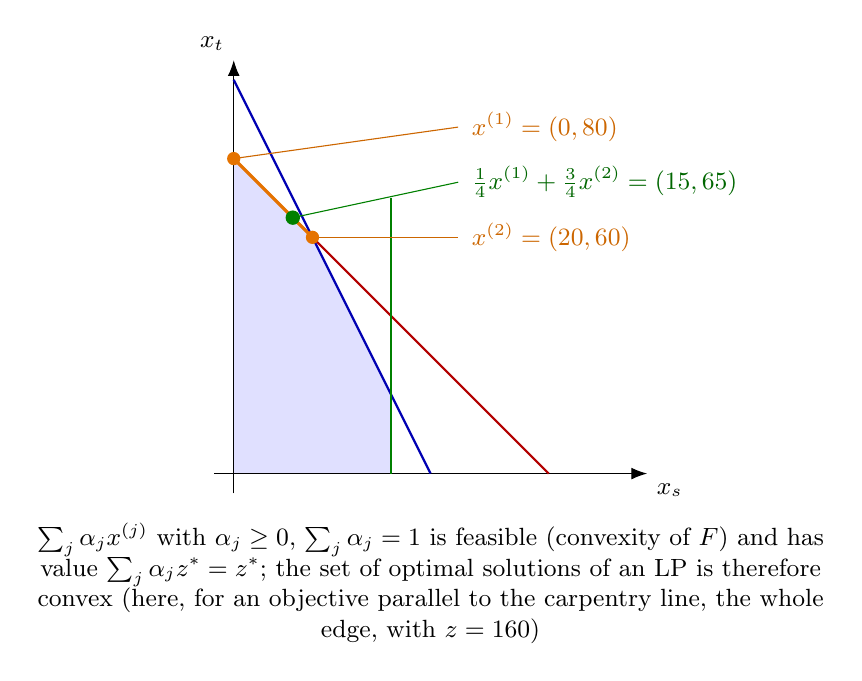
\begin{tikzpicture}[x=0.05cm, y=0.05cm, every node/.style={font=\small}, >={Latex[length=2mm]}]
	\fill[blue!12] (0,0) -- (40,0) -- (40,20) -- (20,60) -- (0,80) -- cycle;
	\draw[->] (-5,0) -- (105,0) node[below right] {$x_s$};
	\draw[->] (0,-5) -- (0,105) node[above left] {$x_t$};
	\draw[blue!70!black, thick] (50,0) -- (0,100);
	\draw[red!70!black, thick] (80,0) -- (0,80);
	\draw[green!50!black, thick] (40,0) -- (40,70);
	\draw[orange!90!black, very thick] (0,80) -- (20,60);
	\draw[orange!80!black, thin] (0,80) -- (57,88);
	\draw[orange!80!black, thin] (20,60) -- (57,60);
	\draw[green!50!black, thin] (15,65) -- (57,74);
	\fill[orange!90!black] (0,80) circle (2.4pt);
	\fill[orange!90!black] (20,60) circle (2.4pt);
	\fill[green!50!black] (15,65) circle (2.6pt);
	\node[orange!80!black, font=\small, anchor=west] at (58,88) {$x^{(1)}=(0,80)$};
	\node[green!40!black, font=\small, anchor=west] at (58,74) {$\tfrac14x^{(1)}+\tfrac34x^{(2)}=(15,65)$};
	\node[orange!80!black, font=\small, anchor=west] at (58,60) {$x^{(2)}=(20,60)$};
	\node[anchor=north, align=flush center, text width=10cm] at (50,-10) {$\sum_j\alpha_jx^{(j)}$ with $\alpha_j\ge0$, $\sum_j\alpha_j=1$ is feasible (convexity of $F$) and has value $\sum_j\alpha_jz^\ast=z^\ast$; the set of optimal solutions of an LP is therefore convex (here, for an objective parallel to the carpentry line, the whole edge, with $z=160$)};
\end{tikzpicture}
\end{document}
